\begin{figure}[htb!]
  \begin{center}
    \resizebox{\textwidth}{!}{
      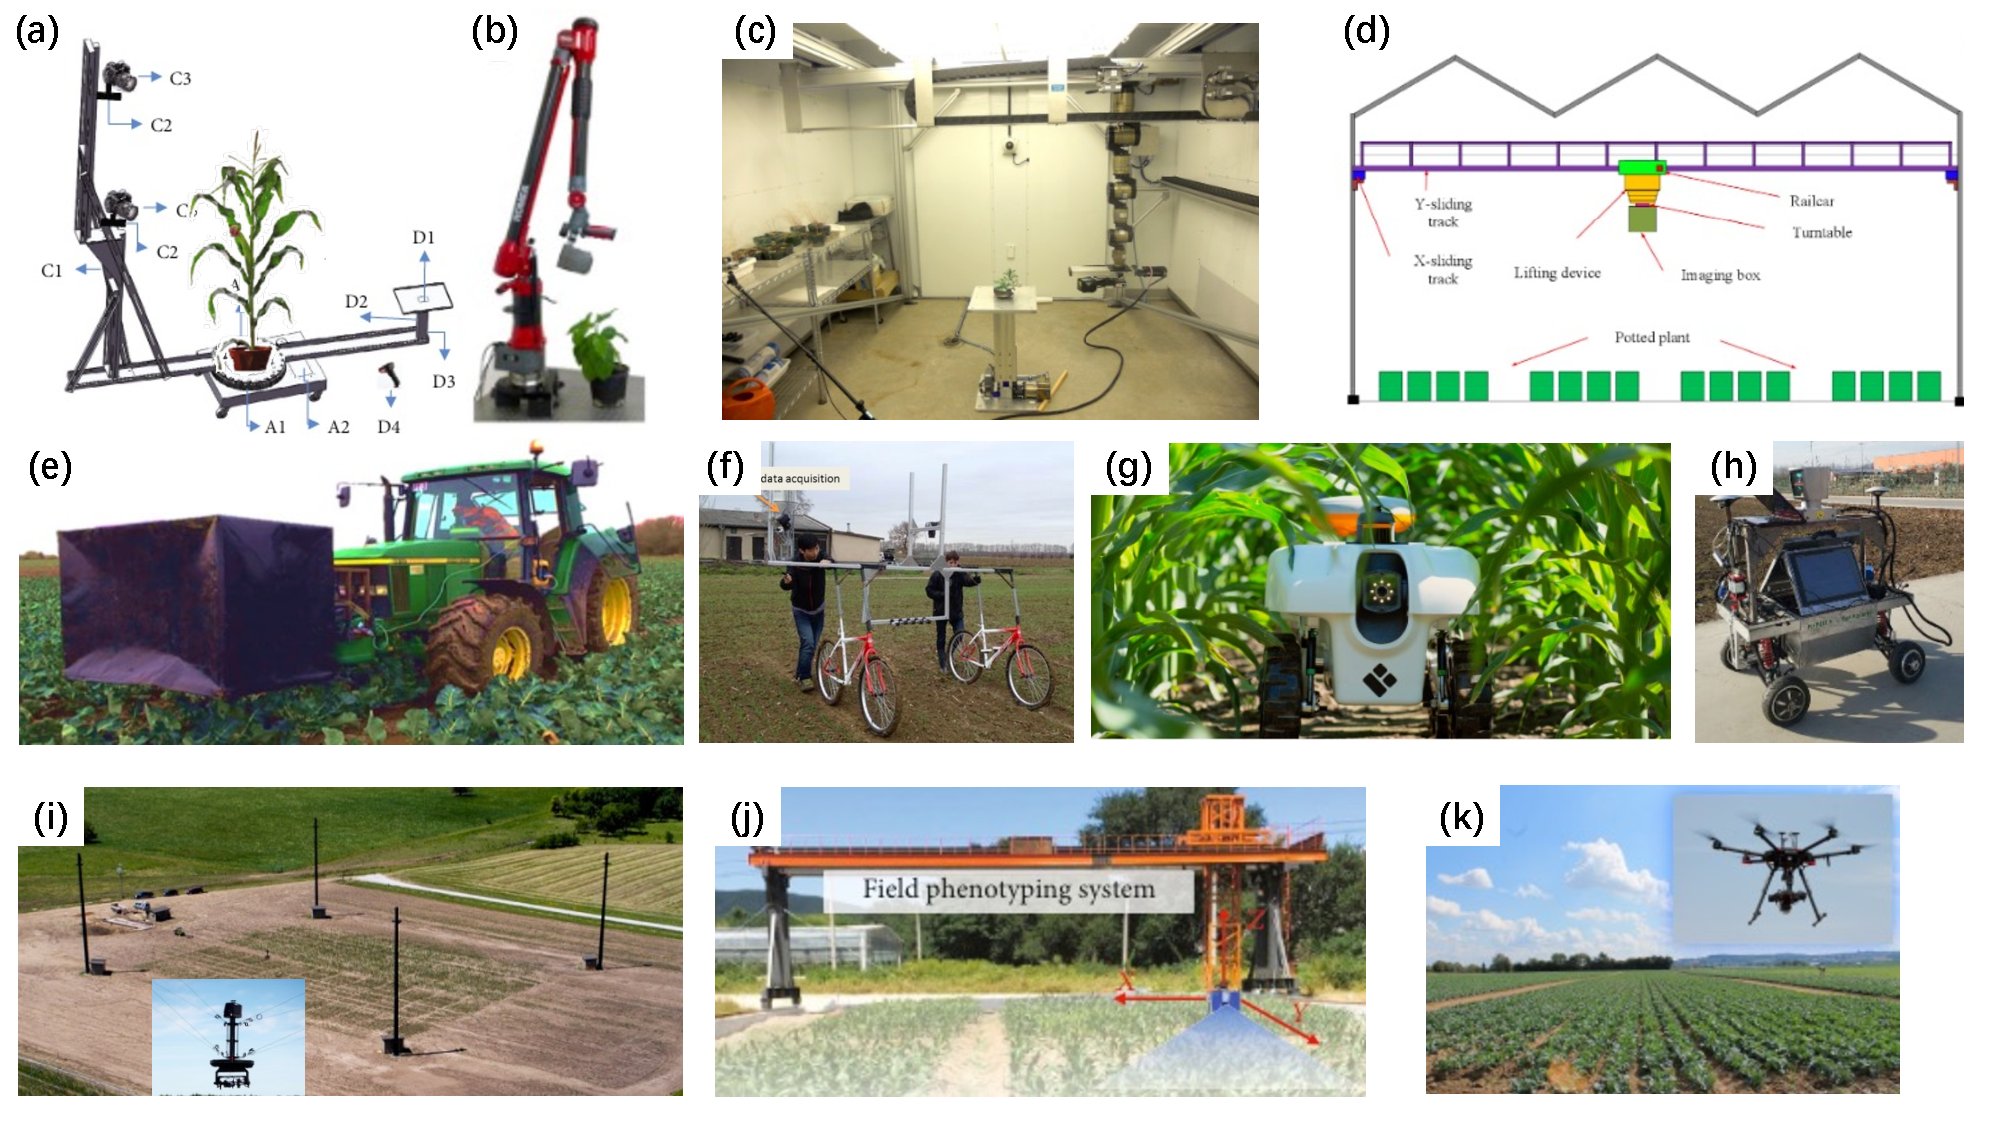
\includegraphics{figures/int/platforms.pdf}
    }
  \end{center}
  \caption[Example of platforms for plant phenotyping]{
    Example of platforms for plant phenotyping in published research. (a-b) self-designed indoor devices \citep{wu_mvs-pheno_2020,schunck_pheno4d_2021}; (c-d) robotic arms in growth chamber or greenhouse \citep{chaudhury_machine_2018, du_greenhouse_2021}; (e) tractor \citep{kusumam_3d_2017}; (f) ground vehicle \citep{liu_estimation_2017}; (g-h) \gls{ugv} \citep{mcguire_high_2021, qiu_field-based_2019}; (i-j) robotic outdoor instruments \citep{bai_nu-spidercam_2019, jin_exploring_2021}; and (k) \gls{uav} \citep{kierdorf_growliflower_2022}
  }
  \label{fig:int1}
\end{figure}